%!TEX TS-program = xelatex
%!TEX encoding = UTF-8

% Unit pembaca Bahasa Indonesia untuk Methods of Algebra, Volume 1.
% Teks sumber: Copyright 2018 Wen-Wei Li, CC BY 4.0.
% Terjemahan ini dilisensikan menurut CC BY 4.0.
% Provenans produksi: OpenAI Codex gpt-5.6-sol, Ultra.

\documentclass[
	colors = true,
	coverpage = coverpage-id-unit-033.tex,
	fontsetup = font-setup-id.tex,
	titlesetup = titles-setup-id.tex,
	CJKthechapter = false
]{AJbook}

% Target-only Indonesian labels for source-class reader interface elements.
% The upstream AJbook.cls remains byte-identical to the frozen source closure.
\renewtcolorbox{wenxintishi}{
	breakable,
	enhanced,
	width = \textwidth,
	colback = white, colbacktitle = white,
	colframe = gray!50, boxrule=0.2mm,
	coltitle = black,
	fonttitle = \sffamily,
	attach boxed title to top left = {yshift=-\tcboxedtitleheight/2, xshift=\tcboxedtitlewidth/4},
	boxed title style = {boxrule=0pt, colframe=white},
	before skip = 0.5cm,
	top = 3mm,
	bottom = 3mm,
	title = {Petunjuk membaca}
}


\makeatletter
\AtBeginDocument{\gdef\mkheader@lemma{\setparms@lemma\@thm{lemma}{theorem}{Lema}}}
\makeatother

\setCJKmainfont[
	Path=../fonts/,
	BoldFont=NotoSansCJKsc-Medium.otf,
	ItalicFont=NotoSansCJKsc-Regular.otf
]{NotoSansCJKsc-Regular.otf}

\newcommand{\BuildDateID}{26 Agustus 2026}
\newcommand{\BuildDateShortID}{2026-08-26}
\AtBeginDocument{\renewcommand{\chaptermark}[1]{\markboth{Bab \thechapter\quad #1}{}}}
\AtBeginDocument{\let\cleardoublepage\clearpage}

\usepackage{mathrsfs}
\usepackage{stmaryrd}
\SetSymbolFont{stmry}{bold}{U}{stmry}{m}{n}
\usepackage{array}
\usepackage{makecell}
\usepackage{tikz-cd}
\usetikzlibrary{positioning, patterns, calc, matrix, shapes.arrows, shapes.symbols}
\usepackage{braids}
\usepackage{tqft}
\usepackage{ytableau}
\usepackage{pgfplots}
\pgfplotsset{compat=1.18}
\usepackage{myarrows}
\usepackage{mycommand}

% Dvipdfmx's extensible rule in \xlongequal is dropped by Poppler.  Keep the
% same labelled equality semantics with a standard embedded math glyph so the
% relation remains visible in both supported renderers.
\renewcommand{\xlongequal}[2][]{\mathrel{\mathop{=}\limits^{\textstyle #2}}}

\usepackage[noautomatic]{imakeidx}
\makeindex[
	columns=2,
	program=makeindex,
	intoc=true,
	title={Indeks Istilah}]
\makeindex[
	columns=3,
	program=makeindex,
	intoc=true,
	name=sym1,
	title={Indeks Simbol}]

\usepackage{xr}
\usepackage[unicode, bookmarksnumbered]{hyperref}
\externaldocument{unit-033-crossrefs}[]
\let\UnitThirtyThreeOriginalRef\ref
\newcommand{\UnitThirtyThreeMarkExternalRef}[1]{%
	\expandafter\def\csname unit033external:#1\endcsname{1}}
\newcommand{\UnitThirtyThreeRef}[1]{%
	\ifcsname unit033external:#1\endcsname
		\begin{NoHyper}\UnitThirtyThreeOriginalRef{#1}\end{NoHyper}%
	\else
		\UnitThirtyThreeOriginalRef{#1}%
	\fi}
\UnitThirtyThreeMarkExternalRef{eg:braid}
\UnitThirtyThreeMarkExternalRef{prop:orbit-decomp}
\UnitThirtyThreeMarkExternalRef{sec:solvable-groups}
\UnitThirtyThreeMarkExternalRef{prop:abelianization}
\UnitThirtyThreeMarkExternalRef{prop:solvable-nilpotent-characterization}
\UnitThirtyThreeMarkExternalRef{eg:dihedral-presentation}
\UnitThirtyThreeMarkExternalRef{prop:Abel-Ruffini}
\hypersetup{
	pdfauthor = {Wen-Wei Li},
	pdftitle = {Metode Aljabar, Jilid 1: Arsitektur Dasar - Unit 33: Grup Simetris},
	pdfsubject = {Terjemahan Bahasa Indonesia independen; Bagian 4.9 lengkap},
	pdfkeywords = {aljabar, teori grup, grup simetris, siklus, grup selang-seling, grup kepang, grup Coxeter, id-ID},
	pdflang = {id-ID},
	CJKbookmarks = true}

\begin{document}
	\hypersetup{pageanchor=false}
	\pagestyle{empty}
	\input{coverpage-id-unit-033.tex}
	\pagestyle{fancy}
	\pagenumbering{roman}
	\setcounter{page}{1}

	\mainmatter
	\hypersetup{pageanchor=true}
	\raggedbottom
	\newgeometry{
		centering,
		textwidth=142mm,
		textheight=198mm,
		headheight=5ex,
		headsep=5ex}
	\setlength{\headwidth}{\textwidth}
	\setcounter{chapter}{4}
	\setcounter{section}{8}
	% Six numbered displays precede Section 4.9 in the complete chapter.
	\setcounter{equation}{6}
	\begingroup
	\setlength{\emergencystretch}{3em}
	\setstretch{1.16}
	\clubpenalty=10000
	\widowpenalty=10000
	\displaywidowpenalty=10000
	\brokenpenalty=10000
	\let\ref\UnitThirtyThreeRef
	% The build script hash-gates this isolated candidate before XeLaTeX.
	\section{Grup Simetris}\label{sec:symmetric-group}
Untuk suatu himpunan $X$, \emph{grup simetris} $\mathfrak{S}_X$ adalah grup semua bijeksi $X \xrightarrow{1:1} X$ terhadap komposisi pemetaan. Grup ini beraksi secara natural dari kiri pada $X$, dan unsur-unsurnya juga disebut permutasi. Bagian ini hanya membahas kasus ketika $n := |X|$ berhingga; dalam hal ini $|\mathfrak{S}_X| = n!$. Lazimnya, unsur-unsur $X$ diidentifikasi dengan $\{1, \ldots, n\}$ dan ditulis $\mathfrak{S}_n := \mathfrak{S}_{\{1, \ldots, n\}}$.

Untuk himpunan $X$ dan $Y$, terdapat pembenaman grup natural $\mathfrak{S}_X \times \mathfrak{S}_Y \hookrightarrow \mathfrak{S}_{X \sqcup Y}$, yang juga dapat ditulis sebagai $\mathfrak{S}_n \times \mathfrak{S}_m \hookrightarrow \mathfrak{S}_{n+m}$. Unsur-unsur $\mathfrak{S}_X$ dan $\mathfrak{S}_Y$ di dalam $\mathfrak{S}_{X \sqcup Y}$ saling komutatif karena unsur-unsur yang mereka gerakkan ``saling lepas''. Hal ini secara natural mengantar kita pada definisi berikut.

\begin{definition}\index{duichengqun@grup simetris (symmetric group)}\index{xunhuan@siklus (cycle)}\index{duihuan@transposisi (transposition)} \index[sym1]{S_n@$\mathfrak{S}_n$}
	Misalkan $a_1, \ldots, a_m$ unsur-unsur berbeda dari $X$. Di dalam grup simetris $\mathfrak{S}_X$, $m$-\emph{siklus} (juga disebut permutasi siklik) $(a_1 \cdots a_m)$ adalah pemetaan $\sigma: X \to X$ berikut:
	\begin{gather*}
		\sigma(a_i) = a_{i+1}, \quad i \in \Z/m\Z, \\
		\sigma(x)=x, \quad x \notin \{a_1, \ldots, a_m\},
	\end{gather*}
	Di sini, demi kemudahan, indeks $\{1, \ldots, m\}$ dipandang sebagai unsur-unsur $\Z/m\Z$, yaitu kelas-kelas kongruensi modulo $m$. Bilangan $m$ disebut panjang siklus tersebut; $2$-siklus $(a b)$ juga disebut \emph{transposisi}. Dua siklus di dalam $\mathfrak{S}_X$, yakni $(a_1 \cdots a_m)$ dan $(b_1 \cdots b_k)$, disebut saling lepas jika $\{a_1, \ldots, a_m\} \cap \{b_1, \ldots, b_k\} = \emptyset$.
\end{definition}
Dari pembahasan sebelumnya, siklus-siklus yang saling lepas komutatif terhadap perkalian. Jelas pula bahwa $\text{ord}((a_1 \cdots a_m)) = m$.

\begin{proposition}[Dekomposisi siklus]\label{prop:cyclic-decomposition}
	Setiap $\sigma \in \mathfrak{S}_X$ dapat dinyatakan sebagai hasil kali siklus-siklus yang saling lepas,
	\[ \sigma = (a_1 a_2 \cdots) (b_1 b_2 \cdots) \cdots \]
	dan siklus-siklus $(a_1 \cdots)$, $(b_1 \cdots)$ di dalamnya unik hingga perubahan urutan. Karena setiap $1$-siklus merupakan unsur identitas, semua siklus panjang satu itu boleh dihilangkan dari hasil kali.
\end{proposition}
\begin{proof}
	Pernyataan ini tidak lain adalah dekomposisi $X$ menjadi orbit-orbit di bawah grup siklik berhingga yang dibangkitkan oleh $\sigma$, yakni $\lrangle{\sigma}$ (Lema \ref{prop:orbit-decomp}). Setiap siklus bersesuaian dengan satu orbit dan mendeskripsikan aksi $\sigma$ pada orbit itu.
\end{proof}

Panjang-panjang siklus $n_1, n_2, \ldots$ yang muncul dalam dekomposisi siklus (termasuk siklus-siklus berpanjang satu) disebut tipe siklus dari $\sigma$, dengan memperhitungkan multiplisitas tetapi mengabaikan urutan. Untuk memperoleh keunikan, kita dapat mengurutkannya sebagai $n_1 \geq n_2 \geq \cdots$; dengan demikian, tipe siklus bersesuaian dengan partisi bilangan bulat $n := |X|$, yakni $n = n_1 + n_2 + \cdots$. Pembahasan tentang orde di atas menyiratkan bahwa orde $\sigma$ sama dengan kelipatan persekutuan terkecil dari $n_1, n_2, \ldots$. \index{fenchai@partisi (partition)}

Berdasarkan hal ini, aksi konjugasi dalam kasus grup simetris dapat dinyatakan dengan rapi.
\begin{lemma}\label{prop:cycle-type}
	Misalkan $\tau = (a_1 a_2 \cdots) (b_1 \cdots) \cdots$ adalah dekomposisi siklus di atas dan $\tau \in \mathfrak{S}_X$. Maka
	\[ \sigma \tau \sigma^{-1} = (\sigma(a_1) \sigma(a_2) \cdots) (\sigma(b_1) \cdots) \cdots. \]
	Sebagai akibatnya, kelas konjugasi unsur $\tau$ ditentukan oleh tipe siklusnya; kelas-kelas konjugasi di dalam $\mathfrak{S}_X$ berkorespondensi satu-satu dengan tipe-tipe siklus $n_1 \geq n_2 \geq \cdots$, yang pada gilirannya berkorespondensi satu-satu dengan partisi bilangan bulat $n = |X|$.
\end{lemma}
\begin{proof}
	Jelas bahwa $\sigma \tau \sigma^{-1}$ memetakan $\sigma(a_i)$ ke $\sigma(a_{i+1})$, memetakan $\sigma(b_j)$ ke $\sigma(b_{j+1})$, dan demikian seterusnya. Karena $\sigma$ bijektif, hal ini menentukan secara unik dekomposisi siklus $\sigma \tau \sigma^{-1}$. Dengan memilih $\sigma$ secara sesuai, $\sigma\tau\sigma^{-1}$ dapat dibuat menjadi sebarang unsur yang memiliki tipe siklus sama dengan $\tau$, dan pembuktian selesai.
\end{proof}

Selanjutnya kita menggunakan notasi $\mathfrak{S}_n$.
\begin{lemma}\label{prop:S_n-generation}
	Grup $\mathfrak{S}_n$ dibangkitkan oleh transposisi-transposisi $\tau_i = (i \quad i+1)$, dengan $1 \leq i < n$.
\end{lemma}
\begin{proof}
	Pandang suatu permutasi $\sigma$ sebagai barisan $\sigma(1), \ldots, \sigma(n)$. Menyatakan $\sigma$ sebagai hasil kali berbagai $\tau_i$ setara dengan mengubah $\sigma(1), \ldots, \sigma(n)$ secara bertahap menjadi $1, \ldots, n$ melalui pertukaran berulang atas suku-suku yang bersebelahan; hal ini tentu dapat dilakukan. Pembuktian yang ketat diserahkan kepada pembaca yang memiliki waktu senggang.
\end{proof}

\begin{lemma}\index[sym1]{sgn@$\sgn$}
	Terdapat homomorfisme grup unik $\sgn: \mathfrak{S}_n \to \{\pm 1\}$ sedemikian sehingga $\sgn((a_1 \cdots a_m)) = (-1)^{m+1}$.
\end{lemma}
\begin{proof}
	Grup $\mathfrak{S}_n$ memiliki aksi kiri natural pada himpunan fungsi $\{ f: \Z^n \to \Z\}$,
	\[ (\sigma f)(x_1, \ldots, x_n) = f(x_{\sigma(1)}, \ldots, x_{\sigma(n)}), \]
	dan aksi ini jelas linear terhadap penjumlahan fungsi secara titik demi titik: $\sigma(f \pm g) = \sigma f \pm \sigma g$. Sekarang perhatikan fungsi
	\[ \Delta(x_1, \ldots, x_n) = \prod_{1 \leq i < j \leq n} (x_j - x_i). \]
	Untuk $\sigma \in \mathfrak{S}_n$, jelas terdapat $\sgn(\sigma) \in \{\pm 1\}$ sedemikian sehingga $\sigma \Delta = \sgn(\sigma)\Delta$. Karena $\Delta$ bukan fungsi nol (sebagaimana terlihat dengan mensubstitusikan $x_i = i$), $\sgn(\sigma)$ ditentukan secara unik; akibatnya, $\sgn: \mathfrak{S}_n \to \{\pm1 \}$ adalah homomorfisme grup. Mudah diperiksa bahwa untuk setiap $1 \leq i < n$ berlaku $\tau_i \Delta = -\Delta$. Semua transposisi saling konjugat, sehingga bagi setiap transposisi $\tau \in \mathfrak{S}_n$ berlaku $\sgn(\tau)=-1$. Dari
	\[(a_1 \cdots a_m) = (a_1 a_m) (a_1 \cdots a_{m-1}) = \cdots = (a_1 a_m) (a_1 a_{m-1}) \cdots (a_1 a_2) \]
	diperoleh $\sgn((a_1 \cdots a_m)) = (-1)^{m+1}$. Keunikan mengikuti dari Proposisi \ref{prop:cyclic-decomposition}.
\end{proof}

\begin{definition}[Grup selang-seling]\index[sym1]{A_n@$\mathfrak{A}_n$}
	\emph{Grup selang-seling} $\mathfrak{A}_n$ didefinisikan sebagai $\Ker[ \mathfrak{S}_n \xrightarrow{\sgn} \{\pm 1\}]$; grup ini merupakan subgrup normal dari $\mathfrak{S}_n$.
\end{definition}
Permutasi yang terletak di dalam $\mathfrak{A}_n$ disebut permutasi genap, sedangkan yang lain disebut permutasi ganjil. Ketika $n > 1$, $(\mathfrak{S}_n : \mathfrak{A}_n) = |\{\pm 1\}| = 2$. Ketika $n \geq 4$, $\mathfrak{A}_n$ tidak abelian; sebagai contoh, $(1 2 3)(1 2 4) = (1 3) (2 4)$, sedangkan $(1 2 4)(1 2 3) = (1 4) (2 3)$.

Kita memerlukan sifat-sifat sederhana berikut:
\begin{itemize}
	\item Untuk grup $\mathfrak{S}_n$, subgrup turunannya (lihat \S\ref{sec:solvable-groups}) $\mathscr{D}^1 \mathfrak{S}_n$ sama dengan $\mathfrak{A}_n$. Untuk $n=1$, hal ini jelas. Berikut penjelasan untuk kasus $n \geq 2$: $\mathfrak{S}_n$ dibangkitkan oleh transposisi-transposisi, dan setiap transposisi konjugat dengan $(1 \; 2)$, sehingga hasil bagi abelian $\mathfrak{S}_n / \mathscr{D}^1 \mathfrak{S}_n$ dibangkitkan oleh bayangan $(1 \; 2)$, yang merupakan unsur berorde dua. Di sisi lain, Lema \ref{prop:abelianization} memberikan homomorfisme surjektif
		\[ \mathfrak{S}_n / \mathscr{D}^1 \mathfrak{S}_n \stackrel{\text{homomorfisme hasil bagi}}{\twoheadrightarrow} \mathfrak{S}_n/\mathfrak{A}_n \simeq \{ \pm 1\}. \]
		Dengan membandingkan orde, homomorfisme di atas ternyata merupakan isomorfisme; jadi $\mathscr{D}^1 \mathfrak{S}_n = \mathfrak{A}_n$.
	\item Semua siklus berpanjang ganjil di dalam $\mathfrak{S}_n$ termuat di dalam $\mathfrak{A}_n$.
	\item Ketika $n \geq 3$, $\mathfrak{A}_n$ dibangkitkan oleh $3$-siklus (yang berbentuk $(i j k)$). Ini karena setiap $\sigma \in \mathfrak{A}_n$ dapat dinyatakan sebagai hasil kali transposisi, dan $\sgn(\sigma)=1$ memastikan bahwa hasil kali tersebut memiliki jumlah suku yang genap. Dengan menggunakan pengamatan berikut,
		\[ (i j)(k l) = \begin{cases}
			1, & \{i,j\} = \{k,l\}, \\
			\text{$3$-siklus}, & \{i,j\} \cap \ \{k,l\}\; \text{tepat satu unsur}, \\
			(i j k) (j k l), & \{i,j\} \cap \ \{k,l\} = \emptyset
		\end{cases} \]
		hasil kali itu dapat ditulis ulang sebagai hasil kali $3$-siklus.
	\item Ketika $n \geq 5$, sebarang dua $3$-siklus $(i j k)$ dan $(i' j' k')$ saling konjugat di dalam $\mathfrak{A}_n$. Pertama, perhatikan bahwa Lema \ref{prop:cycle-type} menyiratkan adanya $\sigma \in \mathfrak{S}_n$ sedemikian sehingga $\sigma (i j k) \sigma^{-1} = (i' j' k')$. Jika $\sigma \in \mathfrak{A}_n$, kita selesai. Jika tidak, ambil unsur-unsur berbeda $l, m \in \{1, \ldots, n\} \smallsetminus \{i,j,k\}$ dan tetapkan $\sigma' := \sigma \cdot (l m) \in \mathfrak{A}_n$; tetap berlaku $\sigma' (i j k) (\sigma')^{-1} = (i' j' k')$.
\end{itemize}
Berikutnya, untuk sebarang permutasi $\sigma$, tulis himpunan titik tetapnya sebagai $\text{Fix}(\sigma) := \left\{ i: \sigma(i)=i \right\}$.

\begin{theorem}[É.\ Galois]\label{prop:A_n-simple}
	Ketika $n \geq 5$, $\mathfrak{A}_n$ adalah grup sederhana.
\end{theorem}
\begin{proof}
	Misalkan $H \lhd \mathfrak{A}_n$ dan $H \neq \{1\}$. Berdasarkan sifat-sifat di atas, cukup mencari sebuah $3$-siklus $\sigma \in H$. Kita mengklaim bahwa suatu $\sigma \in H \smallsetminus \{1\}$ yang memaksimumkan $\left|\text{Fix}(\sigma)\right|$ memiliki sifat ini.
	
	Jika dekomposisi siklus $\sigma$ hanya memuat transposisi, dekomposisi itu memiliki sekurang-kurangnya dua suku, katakanlah $(i j) (k l)$, dengan $\{i,j\} \cap \{k,l\} = \emptyset$. Karena $n \geq 5$, kita dapat mengambil $r \notin \{i,j,k, l\}$ dan mendefinisikan
	\begin{equation}\label{eqn:tau-sigma-simple}
		\tau := (k l r), \quad \sigma' := [\tau, \sigma] = \tau\sigma\tau^{-1}\sigma^{-1} \in H \quad (\because H \lhd \mathfrak{A}_n).
	\end{equation}
	Dapat diperiksa langsung bahwa $i,j \in \text{Fix}(\sigma') \smallsetminus \text{Fix}(\sigma)$, bahwa $\sigma'(k) = r \neq k$, dan bahwa
	\[ \text{Fix}(\sigma) \smallsetminus \{r\} = \text{Fix}(\sigma) \smallsetminus \{k, l, r\} = \text{Fix}(\sigma) \cap \text{Fix}(\tau) \subset \text{Fix}(\sigma'). \]
	Secara keseluruhan, $\left|\text{Fix}(\sigma')\right| > \left|\mathrm{Fix}(\sigma)\right|$, suatu kontradiksi.
	
	Misalkan dekomposisi siklus $\sigma$ memuat suku berpanjang $>2$, yakni $(i j k \cdots)$. Jika $\sigma = (i j k)$, kita telah memperoleh $3$-siklus yang dicari. Jika tidak, karena $\sigma$ tidak mungkin berupa $4$-siklus, $\sigma$ menggerakkan, selain $i,j,k$, sekurang-kurangnya dua unsur berbeda $r,l$. Sekali lagi, melalui \eqref{eqn:tau-sigma-simple}, definisikan $\sigma' \in H$. Dapat diperiksa bahwa $j \in \text{Fix}(\sigma')$, bahwa $\sigma'(k) = l \neq k$, dan bahwa
	\[ \text{Fix}(\sigma) = \text{Fix}(\sigma) \smallsetminus \{k,l,r\} = \text{Fix}(\sigma) \cap \text{Fix}(\tau) \subset \text{Fix}(\sigma'). \]
	Sekali lagi kita memperoleh kontradiksi $\left|\text{Fix}(\sigma')\right| > \left|\mathrm{Fix}(\sigma)\right|$. Ini membuktikan klaim.
\end{proof}

Ketika $n \geq 5$, $\mathfrak{A}_n$ adalah grup sederhana nonabelian, sehingga grup ini harus sama dengan subgrup turunannya sendiri, $\mathscr{D}^1 \mathfrak{A}_n$. Akibat berikut merupakan kunci teori grup bagi pembuktian bahwa persamaan berderajat lima atau lebih tidak dapat diselesaikan dengan radikal (Teorema \ref{prop:Abel-Ruffini}).
\begin{corollary}\label{prop:S_n-unsolvable}\index{kejiequn@grup solvabel (solvable group)}
	Ketika $n \geq 5$, untuk setiap $i \geq 1$ berlaku $\mathscr{D}^i \mathfrak{S}_n = \mathfrak{A}_n$; akibatnya, ketika $n \geq 5$, $\mathfrak{S}_n$ tidak solvabel.
\end{corollary}
\begin{proof}
	Kita telah mengetahui bahwa $\mathscr{D}^1 \mathfrak{S}_n = \mathfrak{A}_n$. Bersama pembahasan sebelumnya, ketika $n \geq 5$, untuk setiap $i \geq 1$ berlaku $\mathscr{D}^i \mathfrak{S}_n = \mathscr{D}^{i-1} \mathfrak{A}_n = \mathfrak{A}_n$. Untuk pernyataan bahwa grup tersebut tidak solvabel, lihat Lema \ref{prop:solvable-nilpotent-characterization}.
\end{proof}

Pembaca dapat memeriksa secara langsung bahwa \[ \mathscr{D}^1 \mathfrak{A}_4 = \left\{\identity, (1 2)(3 4), (1 3) (2 4), (1 4)(2 3)\right\} , \] yang isomorfik dengan $(\Z/2\Z)^2$. Jadi, ketika $n < 5$, $\mathfrak{S}_n$ memang solvabel.

Selanjutnya kita mempelajari presentasi $\mathfrak{S}_n$. Untuk itu, kita sekaligus mempertimbangkan grup kepang yang disebutkan dalam Contoh \ref{eg:braid}, yakni $\mathcal{B}_n$. Berikut ringkasan singkat konstruksi sebelumnya: secara visual, unsur-unsur $\mathcal{B}_n$ adalah kepang yang dibentuk oleh semua konfigurasi $n$ untai, dengan kepang-kepang yang dapat dideformasi secara kontinu di dalam ruang $\R^3$ (titik-titik ujung tetap dan untai-untai tidak dipotong) dipandang ekuivalen. Kepang dapat digambarkan, misalnya, sebagai berikut (untuk $n=2,3$):
\begin{center}
\begin{tikzpicture}[baseline=(braid)]
	\braid[style strands={1}, style strands={2}] (braid) s_1;
	\end{tikzpicture} \qquad 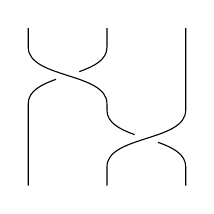
\begin{tikzpicture}[baseline=(braid), yscale=0.8]
	\braid[style strands={1}, style strands={2}, style strands={3}] (braid)  s_1 s_2^{-1};
\end{tikzpicture}\end{center}
Perkalian di dalam grup kepang dilakukan dengan menyambungkan kepang dari atas ke bawah, misalnya
\begin{center}
\begin{tikzpicture}[baseline=(braid)]
	\braid[style strands={1}, style strands={2}] (braid) s_1;
	\end{tikzpicture} \quad $\bullet$ \quad 
\begin{tikzpicture}[baseline=(braid)]
	\braid[style strands={1}, style strands={2}] (braid) s_1^{-1};
	\end{tikzpicture} \quad $=$ \quad 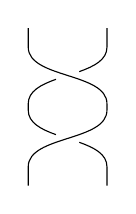
\begin{tikzpicture}[baseline=(braid), yscale=0.8]
	\braid[style strands={1}, style strands={2}] (braid) s_1 s_1^{-1};
	\end{tikzpicture} \quad $\xlongequal{\text{diluruskan}}$ \quad
	\begin{tikzpicture}[baseline=(M), yscale=0.8]
	\draw (0,1) -- (0,-1);
	\draw (1,1) -- (1,-1);
	\coordinate (M) at (0,0);
\end{tikzpicture}\end{center}
Hukum asosiatif langsung terlihat, dan unsur identitas $\mathcal{B}_n$ adalah $n$ untai sejajar $\vert \cdots \vert$. Pencerminan diagram kepang terhadap sumbu horizontal memberikan inversnya; mengapa demikian? Perhatikan dengan saksama gambar di atas.

``Peletakan berdampingan'' secara horizontal atas dua kepang menghasilkan homomorfisme grup $\mathcal{B}_n \times \mathcal{B}_m \to \mathcal{B}_{n+m}$.

Jelas bahwa $\mathcal{B}_1 = \{1\}$. Berikutnya, andaikan $n \geq 2$. Untuk $1 \leq i < n$, definisikan unsur $\sigma_i \in \mathcal{B}_n$ sedemikian sehingga pola persilangan untai ke-$i$ dan ke-$i+1$ adalah
\begin{center} 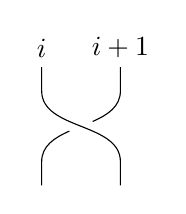
\begin{tikzpicture}
	\braid[style strands={1}, style strands={2}] (braid) s_1;
	\node[above] at (braid-1-s) {$i$};
	\node[above] at (braid-2-s) {$i+1$};
\end{tikzpicture} \end{center}
sedangkan untai-untai lainnya tidak saling berpilin. Mudah dilihat bahwa ketika $|i-j| > 1$, untai-untai yang dipengaruhi oleh $\sigma_i$ dan $\sigma_j$ saling lepas, sehingga $\sigma_i \sigma_j = \sigma_j \sigma_i$. Di sisi lain, ``persamaan Yang--Baxter''
\[ 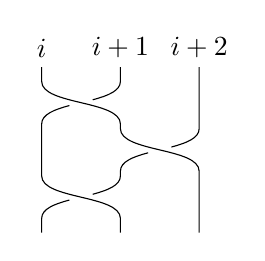
\begin{tikzpicture}[yscale=0.6, baseline=(braid)]
	\braid[style strands={1}, style strands={2}, style strands={3}] (braid) s_1 s_2 s_1;
	\node[above] at (braid-1-s) {$i$};
	\node[above] at (braid-2-s) {$i+1$};
	\node[above] at (braid-3-s) {$i+2$};
	\end{tikzpicture}
	\qquad = \qquad
	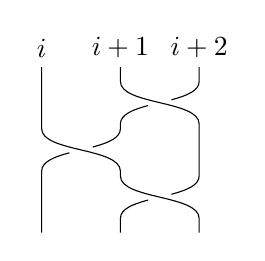
\begin{tikzpicture}[yscale=0.6, baseline=(braid)]
	\braid[style strands={1}, style strands={2}, style strands={3}] (braid) s_2 s_1 s_2;
	\node[above] at (braid-1-s) {$i$};
	\node[above] at (braid-2-s) {$i+1$};
	\node[above] at (braid-3-s) {$i+2$};
\end{tikzpicture} \]
menunjukkan bahwa $\sigma_i \sigma_{i+1} \sigma_i = \sigma_{i+1} \sigma_i \sigma_{i+1}$ selalu berlaku untuk $1 \leq i < n-1$. Pembaca dipersilakan mencoba memahami secara intuitif bahwa
\begin{inparaenum}[(a)]
	\item unsur-unsur $\sigma_1, \ldots, \sigma_{n-1}$ membangkitkan $\mathcal{B}_n$,
	\item relasi-relasi $|i-j| > 1 \implies \sigma_i \sigma_j = \sigma_j \sigma_i$ dan $\sigma_i \sigma_{i+1} \sigma_i = \sigma_{i+1} \sigma_i \sigma_{i+1}$ sepenuhnya mendeskripsikan struktur $\mathcal{B}_n$.
\end{inparaenum}
Pernyataan yang lebih ringkas menggunakan presentasi grup
\begin{equation}\label{eqn:braid-presentation} \left\langle \sigma_1, \ldots, \sigma_{n-1} \Biggr| \begin{array}{ll}
	\sigma_i \sigma_j = \sigma_j \sigma_i, & |i-j| > 1 \\
	\sigma_i \sigma_{i+1} \sigma_i = \sigma_{i+1} \sigma_i \sigma_{i+1}, & 1 \leq i < n-1
	\end{array} \right\rangle \rightiso \mathcal{B}_n. \end{equation}

Presentasi ini dapat diturunkan dari interpretasi topologis $\mathcal{B}_n$, atau dapat langsung dijadikan definisi kombinatorial grup kepang. Perhatikan bahwa $\mathcal{B}_2 \simeq \Z$, sedangkan ketika $n \geq 3$, $\mathcal{B}_n$ merupakan grup tak hingga nonabelian.

Sekarang kita hubungkan $\mathcal{B}_n$ dengan $\mathfrak{S}_n$. Untuk setiap kepang $x \in \mathcal{B}_n$, definisikan $\sigma \in \mathfrak{S}_n$ yang bersesuaian sedemikian sehingga pada diagram kepang, lintasan dari ujung bawah $i$ berakhir di ujung atas $\sigma(i)$, seperti berikut:
\begin{center}\begin{tikzpicture}[scale=0.5]
	\node (S) at (-1.7, 1) {$\sigma(i)$};
	\node (E) at (1.7, -1) {$i$};
	\draw (S) -- (E) node[midway, fill=white, anchor=center, sloped] {$\cdots$};
\end{tikzpicture}\end{center}
Jelas bahwa hal ini memberikan homomorfisme grup $\mathcal{B}_n \to \mathfrak{S}_n$ yang membuat diagram
\[\begin{tikzcd}
	\mathcal{B}_n \times \mathcal{B}_m \arrow[r] \arrow[d] & \mathcal{B}_{n+m} \arrow[d] \\
	\mathfrak{S}_n \times \mathfrak{S}_m \arrow[r] & \mathfrak{S}_{n+m}
\end{tikzcd}\]
komutatif, dan memetakan $\sigma_i \in \mathcal{B}_n$ ke transposisi
\[ \tau_i := (i \quad i+1) \in \mathfrak{S}_n, \quad 1 \leq i < n. \]
Lema \ref{prop:S_n-generation} menyatakan bahwa transposisi-transposisi itu membangkitkan $\mathfrak{S}_n$. Jika kita mulai dari presentasi $\mathcal{B}_n$ dalam \eqref{eqn:braid-presentation}, pertama-tama kita dapat memeriksa relasi-relasi berikut di dalam $\mathfrak{S}_n$:
\begin{gather*}
	|i-j| > 1 \implies \tau_i \tau_j = \tau_j \tau_i, \\
	\tau_i^2 = 1, \quad 1 \leq i < n, \\
	\tau_i \tau_{i+1} \tau_i = \tau_{i+1} \tau_i \tau_{i+1} = (i \quad i+2), \quad 1 \leq i < n-1.
\end{gather*}
Jadi, $\sigma_i \mapsto \tau_i$ menentukan suatu homomorfisme $\mathcal{B}_n \to \mathfrak{S}_n$. Hal ini memunculkan pertanyaan yang wajar: apakah relasi-relasi tersebut memberikan presentasi $\mathfrak{S}_n$?

Untuk menghindari ketaksaan, gunakan simbol baru $\tilde{\tau}_i$ di dalam ketiga keluarga relasi di atas. Secara bersama-sama, relasi-relasi itu dapat ditulis dalam bentuk ekuivalen
\begin{equation}\label{eqn:S_n-presentation}\begin{gathered}
	\tilde{\tau}_i^2 = 1, \quad 1 \leq i < n \\
	|i-j| > 1 \implies (\tilde{\tau}_i \tilde{\tau}_j)^2 = 1, \\
	(\tilde{\tau}_i \tilde{\tau}_{i+1})^3 = 1, \quad 1 \leq i < n-1.
\end{gathered}\end{equation}
Definisikan $\mathfrak{S}'_n := \lrangle{\tilde{\tau}_1, \ldots, \tilde{\tau}_{n-1} \big| \text{memenuhi}\; \eqref{eqn:S_n-presentation} }$, serta tetapkan $\mathfrak{S}'_1 := \{1\}$. Dengan demikian, terdapat homomorfisme grup $\mathcal{B}_n \twoheadrightarrow \mathfrak{S}'_n \twoheadrightarrow \mathfrak{S}_n$ yang memenuhi $\sigma_i \mapsto \tilde{\tau}_i \mapsto \tau_i$. Beralih dari $\mathcal{B}_n$ ke $\mathfrak{S}'_n$ berarti mengabaikan lilitan ganda
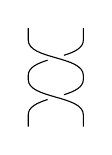
\begin{tikzpicture}[baseline=(braid), yscale=0.5, xscale=0.7]
	\braid[style strands={1}, style strands={2}] (braid) s_1 s_1;
\end{tikzpicture}.

\begin{theorem}\label{prop:S_n-presentation}
	Pemetaan $\mathfrak{S}'_n \to \mathfrak{S}_n$ merupakan isomorfisme; dengan kata lain, \eqref{eqn:S_n-presentation} memang memberikan presentasi $\mathfrak{S}_n$.
\end{theorem}
\begin{proof}
	Karena $\mathfrak{S}'_n \to \mathfrak{S}_n$ adalah homomorfisme surjektif, cukup dibuktikan secara rekursif bahwa $|\mathfrak{S}'_n| \leq n!$. Kasus $n=1,2$ trivial, sehingga selanjutnya andaikan $n > 2$. Presentasi \eqref{eqn:S_n-presentation} memberikan homomorfisme natural $\mathfrak{S}'_{n-1} \to \mathfrak{S}'_n$. Kita belum mengetahui apakah homomorfisme ini injektif, tetapi kita selalu dapat membiarkan $\mathfrak{S}'_{n-1}$ beraksi pada $\mathfrak{S}'_n$ melalui perkalian kanan dan mempelajari orbit-orbitnya. Kita mengklaim bahwa
	\[ \mathfrak{S}'_n = 1 \cdot \mathfrak{S}'_{n-1} \cup \tilde{\tau}_{n-1}\mathfrak{S}'_{n-1} \cup \cdots \cup (\tilde{\tau}_1 \cdots \tilde{\tau}_{n-1} \mathfrak{S}'_{n-1}), \]
	jika kesamaan ini berlaku, segera diperoleh $|\mathfrak{S}'_n| \leq n |\mathfrak{S}'_{n-1}| \leq n(n-1)! = n!$.
	
	Cukup dibuktikan bahwa ruas kanan kesamaan tersebut tertutup terhadap perkalian kiri oleh setiap $\tilde{\tau}_i$. Perhatikan $\tilde{\tau}_i (\tilde{\tau}_j \cdots \tilde{\tau}_{n-1}) \mathfrak{S}'_{n-1}$: ketika $i=j-1$ atau $i=j$, ketertutupan langsung terlihat ($\tilde{\tau}_j^2 = 1$); ketika $i < j-1$, dengan \eqref{eqn:S_n-presentation}, $\tilde{\tau}_i$ dapat digeser ke kanan dan diserap ke dalam $\mathfrak{S}'_{n-1}$, sehingga ketertutupan tetap berlaku. Jadi, selanjutnya andaikan $i>j$. Kita menggunakan relasi kedua dalam \eqref{eqn:S_n-presentation} untuk menggeser $\bm{\tilde{\tau}_i}$ ke kanan (jenis hurufnya diubah untuk memberi penekanan), hingga diperoleh
	\[ \cdots \tilde{\tau}_{i-2} \bm{\tilde{\tau}_i} \tilde{\tau}_{i-1} \tilde{\tau}_i \tilde{\tau}_{i+1} \cdots \mathfrak{S}'_{n-1}. \]
	Kemudian, gunakan relasi ketiga dalam \eqref{eqn:S_n-presentation} (atau bentuknya dalam \eqref{eqn:braid-presentation}) untuk mengubah ungkapan itu menjadi
	\[ \cdots \tilde{\tau}_{i-2} \tilde{\tau}_{i-1} \tilde{\tau}_i \bm{\tilde{\tau}_{i-1}} \tilde{\tau}_{i+1} \cdots \mathfrak{S}'_{n-1}. \]
	Unsur $\bm{\tilde{\tau}_{i-1}}$ yang ditandai di atas dapat digeser terus ke kanan hingga terserap ke dalam $\mathfrak{S}'_{n-1}$; jadi, ketertutupan terhadap perkalian kiri yang diperlukan telah terbukti.
\end{proof}

Presentasi \eqref{eqn:S_n-presentation} menunjukkan bahwa grup simetris termasuk dalam suatu kelas konstruksi yang disebut grup Coxeter. Grup-grup ini memiliki presentasi berbentuk $W = \lrangle{S \big| (st)^{m(s,t)}=1, \; s,t \in S}$, dengan
\begin{compactitem}
	\item $S$ sebuah himpunan berhingga,
	\item $m: S \times S \to \Z_{\geq 1} \sqcup \{\infty\}$ (nilai $\infty$ berarti tidak ada relasi),
	\item $\forall s,t \in S, \; m(s,t)=m(t,s)$,
	\item $s=t \iff m(s,t)=1$.
\end{compactitem}
Contoh \ref{eg:dihedral-presentation} menunjukkan bahwa grup dihedral $D_{2n}$ juga memiliki presentasi semacam ini. Grup Coxeter merupakan perangkat yang tak tergantikan dalam studi grup Lie, aljabar Lie, dan teori representasi terkait. \index{grup Coxeter (Coxeter group)}

	\endgroup

	\begingroup
	\setlength{\emergencystretch}{3em}
	\par\bigskip
	\let\clearpage\relax
	\let\cleardoublepage\relax
	\IfFileExists{\jobname.ind}{
		\begingroup
		\renewenvironment{theindex}
			{\par\smallskip
			 \phantomsection
			 \pdfbookmark[0]{Indeks Istilah}{unit033-term-index}
			 \noindent{\small\sffamily\bfseries Indeks Istilah.}\enspace
			 \small
			 \let\UnitThirtyThreeIndexPar\par
			 \let\par\relax
			 \def\item{\unskip\hspace{1.25em}\penalty0}
			 \let\indexspace\relax}
			{\let\par\UnitThirtyThreeIndexPar\par}
		\input{\jobname.ind}
		\endgroup
	}{}
	\IfFileExists{sym1.ind}{
		\begingroup
		\renewenvironment{theindex}
			{\par\smallskip
			 \phantomsection
			 \pdfbookmark[0]{Indeks Simbol}{unit033-symbol-index}
			 \noindent{\small\sffamily\bfseries Indeks Simbol.}\enspace
			 \small
			 \let\UnitThirtyThreeSymbolIndexPar\par
			 \let\par\relax
			 \def\item{\unskip\hspace{1.25em}\penalty0}
			 \let\indexspace\relax}
			{\let\par\UnitThirtyThreeSymbolIndexPar\par}
		\input{sym1.ind}
		\endgroup
	}{}
	\endgroup
\end{document}
